\documentclass[a4paper]{article}

\usepackage[francais]{babel}
%\usepackage{amsmath}
\usepackage{graphicx}
\usepackage{fontspec}
%\usepackage{listings}
%\usepackage{moreverb}
%\usepackage{color}
%\usepackage[colorinlistoftodos]{todonotes}
%\usepackage[labelformat=empty]{caption}
\usepackage[textheight=25cm]{geometry}
\usepackage{hyperref}

\renewcommand{\thefootnote}{\alph{footnote}}
%\setlength{\textwidth}{420 pt} 

\title{La guerre de Twitch contre le viewbotting}

\author{Alexandre MOEVI}

\date{\today}

\setlength{\parskip}{1em}

\begin{document}
\maketitle

\section{Twitch, acteur majeur du \textit{live streaming}}
\subsection{Qu'est-ce que le \textit{live streaming} ?}
Avant tout chose, une introduction ou un rappel de ce qu'est le \textit{live streaming} ainsi que de son vocabulaire me semble nécessaire. La plupart de ce vocabulaire est en anglais et, même s'il existe des traductions françaises plus ou moins officielles, ma préférence pour ce mémoire ira aux termes anglophones (question d'habitude).

Un utilisateur diffuse du contenu en ligne et en direct (ou en léger différé) à partir de son ordinateur ou de son smartphone. On dit alors qu'il est le \textit{broadcaster}, le \textit{caster} ou le \textit{streamer}. Pour ce faire, il va utiliser des logiciels de streaming afin de configurer l'envoi du flux (débit binaire du flux, résolution de la vidéo, volume sonore\ldots).

Le principal intérêt du live streaming est que les autres utilisateurs, les \textit{viewers} ou spectateurs, regardent le contenu en direct sur la plate-forme et peuvent interagir avec le streamer à travers un chat. 

Streamer ou viewer, les utilisateurs doivent d'abord créer un compte sur la plate-forme et ils sont identifiés par leur pseudonyme. Par plate-forme, on entend le site web et l'application sur les différents supports. Dans le cas de Twitch, une application est disponible sur smartphones et tablettes. Twitch est également disponible sur les consoles \textit{Xbox One} et \textit{PlayStation 4}. Il est possible de directement diffuser à partir de ces consoles, sans configuration spéciale nécessaire.

\subsection{La \textit{success story} Twitch}
Si le site twitch.tv n'est lancé qu'en juin 2011, son histoire commence quatre ans plutôt. En 2007, Justin Kan, Emmett Shear, Michael Seibel et Kyle Vogt lancent la plateforme de live streaming Justin (le site web justin.tv et l'application mobile). Justin était divisé en plusieurs catégories (ou sections), chaque catégorie étant un type de diffusion en direct. On pouvait voir une épreuve de jet-ski dans la catégorie \textit{Sports}, le quotidien de hamsters dans la section \textit{Animals} ou un artiste amateur peindre une œuvre du début jusqu'à la fin dans \textit{Arts}. Mais la catégorie qui se distingue particulièrement est la section jeux vidéo (\textit{Gaming}).

Très vite, les joueurs et les entreprises du marché vidéoludique utilisent la plate-forme Justin pour la diffusion de \textit{playthroughs}\footnote{Un playthrough est une vidéo produite par un joueur qui montre le déroulement d'un jeu en entier ou en partie.} et de compétitions \textit{e-sport}\footnote{À cette époque, les tournois internationaux de \textit{StarCraft} et \textit{Counter-Strike} étaient déjà dotés de plusieurs dizaines de milliers d'euros. L'enjeu pour les joueurs professionnels était déjà conséquent\ldots}. Le succès de la section Gaming est tel que les dirigeants de justin.tv ont décidé en 2011 de séparer cette section du reste du site et d'en faire une plate-forme à part entière. C'est l'acte de naissance de Twitch\cite{BW2011}.

Twitch continue sa croissance florissante et domine largement le marché du live streaming de jeux vidéo, loin devant ses concurrents directs Hitbox et Azubu. En février 2014, Twitch est le quatrième consommateur de bande passante aux États-Unis avec 1,8\% du trafic, devant Facebook, Amazon ou Valve\cite{Polygon2014}. 

Le succès de Twitch est également un succès communautaire. L'expérience \textit{Twitch Plays Pokémon} (TPP), dans laquelle les utilisateurs contrôlent le héros du jeu Pokémon via les messages envoyés dans le chat, est relayée par des médias mainstream (BBC, CNN, Le Monde). La fin du jeu est atteinte après deux semaines, 36 millions de vues (pic d'audience à 121000 personnes), 122 millions de messages et un million de participants\cite{Gadget2014}. TPP a donné naissance à des variantes improbables comme \textit{Twitch Plays Tamagotchi} ou \textit{Twitch Installs Arch Linux}\footnote{Pour plus de détails, on peut lire cet article de presse remontant à novembre 2015 : \href{http://www.pcworld.com/article/3001378/operating-systems/after-beating-dark-souls-and-pokemon-twitch-is-installing-arch-linux.html}{\textit{After beating Dark Souls and Pokemon, Twitch is installing Arch Linux}}. Malheursement, le stream (\href{https://www.twitch.tv/twitchinstallsarchlinux}{\texttt{twitch.tv/twitchinstallsarchlinux}}) n'est plus actif depuis quelques mois.}. Les émoticônes disponibles\footnote{Le site \href{https://twitchemotes.com/}{\texttt{twitchemotes.com}} contient la liste exhaustive des émoticônes officielles de Twitch. Pour les plus bavards, le lien \href{https://nightdev.com/betterttv/faces.php}{\texttt{nightdev.com/betterttv/faces.php}} recense des émoticônes de l'extension Better Twitch TV.} et le dialecte développé sur Twitch\footnote{Des expressions comme « Never Lucky 
\includegraphics[width=0.4cm]{BabyRage.jpg} », « NA PLAYS 
\includegraphics[width=0.3cm]{4Head.png} », « Saved 
\includegraphics[width=0.4cm]{KappaRoss.png} » ou « HOLD THE LINE 
\includegraphics[width=0.4cm]{WutFace.png} » sont incompréhensibles pour les non-initiés.} renforcent le sentiment d'appartenance à la communauté. 

Les chiffres de la croissance de Twitch donnent le vertige. En moyenne sur l'année 2015, 550000 personnes étaient en train de regarder un stream à n'importe quel moment, avec un pic d'audience à 2 millions de spectateurs le 23 août. Un utilisateur regarde par mois 421 minutes de contenu Twitch (contre 291 minutes de Youtube). 9 milliards de messages ont été envoyés sur les chats, ce qui donne près de 300 messages par seconde\cite{Retro2015}.

Des chiffres qui ont attiré l'\oe{}il des mastodontes du web, Amazon et Google. Après plusieurs mois de tractations avec le géant de Mountain View, c'est finalement Amazon qui rachète Twitch fin août 2014 pour un peu moins d'un milliard d'euros. Google riposte et crée un an plus tard sa plate-forme de streaming \textit{YouTube Gaming}, un potentiel \textit{Twitch-killer} vu les moyens dont dispose la maison-mère\cite{Echos2015}. Une étude de février 2016 montre que la moitié des « gamers » américains regardent regulièrement des vidéos vidéoludiques sur YouTube\footnote{L'étude parle du YouTube classique et donc de l'hébergement de vidéos. Aucune étude comparative n'a été faite pour l'instant entre les deux plate-formes de streaming Youtube Gaming et Twitch.} alors que seuls 21\% d'entre eux vont sur Twitch. Pour la France, on est à 43\% pour YouTube et un gamer sur dix pour Twitch\cite{Newzoo2016}. Le but pour Google est d'inciter les gamers à rester dans l'univers Youtube.

Quant à Justin, la plate-forme a fermé ses portes en août 2014. Cette fermeture a pour but de concentrer tous les mooyens techniques et humains sur Twitch pour ceratins, pour d'autres l'objectif était de se débarrasser du boulet qu'est devenu Justin avant un rachat de Twitch\footnote{La plate-forme Justin était connu pour être le paradis des diffusions illégales. Des ayants droits sont allés jusqu'à une action en justice, l'UFC (\textit{Ultimate Fighting Championship}) en janvier 2011 par exemple}. Twitch qui se revendiquait comme une plateforme 100\% jeu vidéo a lancé en octobre 2015 la section \textit{Twitch Creative} qui permet aux utilisateurs de diffuser du contenu créatif (peinture, musique, cuisine ou même de la programmation)\ldots comme le faisait son prédécesseur Justin. 
\newpage 
\section{Le \textit{viewbotting}}

\subsection{Simuler la présence de spectateurs}

Le succès de Twitch et des plus gros \textit{streamers} sur cette plateforme ont motivé des dizaines de milliers de personnes (dont moi-même) à se lancer dans l'aventure du \textit{live streaming}. Vue la forte concurrence sur Twitch, certaines d'entre elles sont prêtes à tout pour obtenir la popularité et la richesse, quitte à utiliser des moyens frauduleux (et pas du tout fair-play).

Dès qu'un stream sur Twitch démarre, on peut observer en bas du flux vidéo, le nombre de spectateurs en train de regarder le stream. Sur une page du site, on peut également voir la liste de tous les streams en direct. La liste est triée par ordre décroissant des viewers, c'est-à-dire que les streams les plus populaires va apparaître en haut de la page.

%Capture d'écran

\begin{figure}[!h]
	\centering
	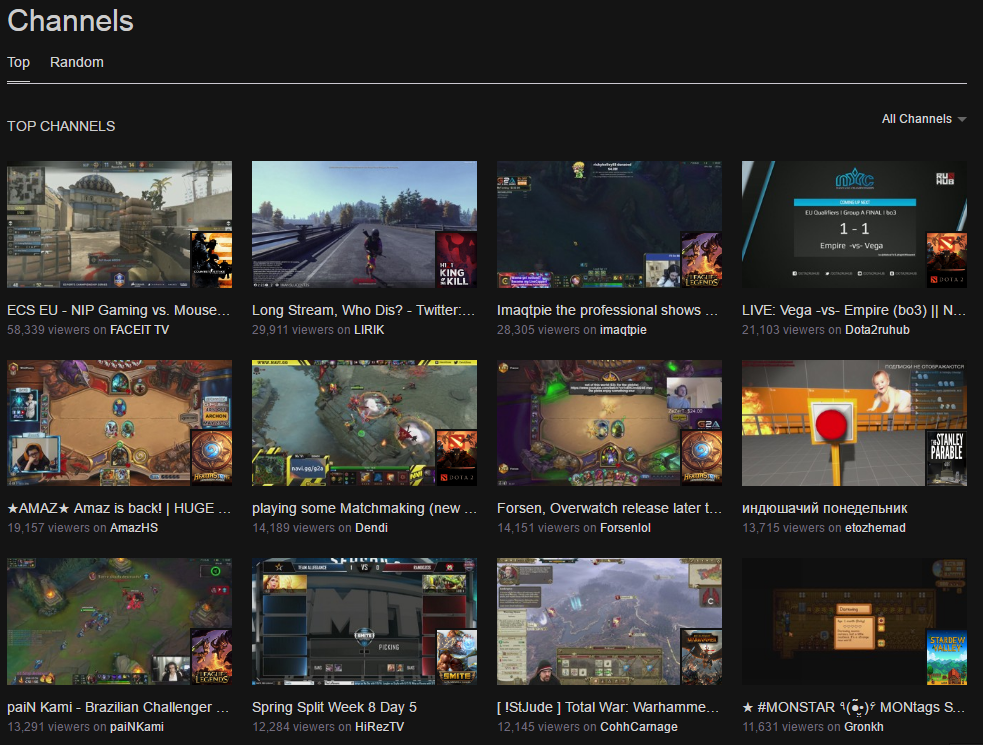
\includegraphics[height=8.5cm]{channels.png}
	\caption{Liste des chaînes en cours de diffusion sur Twitch (\href{https://www.twitch.tv/directory/all}{\texttt{twitch.tv/directory/all}}). Apparaître en haut de cette page est le Graal de certains streamers en herbe.}
\end{figure}

Le jeu est donc de gonfler le nombre de spectateurs afin d'apparaître au sommet de l'affiche et d'attirer de nouveaux spectateurs par effet boule de neige (plus de gens regardent un stream, plus ce stream a de chances d'attirer de nouvelles personnes). L'enjeu est également financier puisque les plus gros streamers signent un contrat avec Twitch pour se partager les revenus générés par la chaîne (abonnements\footnote{Un utilisateur peut s'abonner à un streamer pour 5 dollars par mois. Ces cinq dollars sont partagés entre le streamer et Twitch (moitié-moitié). Les streamers les plus populaires ont plus de 1500 abonnés, ce qui fait un revenu mensuel de 3750 dollars\ldots}, dons des spectateurs\footnote{Encore une fois, pour les streamers les plus en vue, c'est le jackpot. Le Suédois Sebastian « \href{https://www.twitch.tv/forsenlol}{Forsen} » Fors peut toucher plus de 18000 dollars de dons en un mois. Ce nombre vient de l'une de ses diffusions où il a affiché un tableau de bord (voir une \href{http://imgur.com/gallery/OLyQNpk}{capture d'écran}).}, publicité\footnote{Les streamers sous contrat avec Twitch peuvent diffuser des publicités sur le stream. Là encore, les revenus venant de ces publicités sont partagés entre le broadcaster et Twitch. Pour plus de détails, voir \href{https://blog.twitch.tv/updates-to-twitch-commercial-policy-a35f5ce89afa}{\textit{Updates to Twitch Commercial Policy}}}.).

Commencer à booster sa chaîne avec des viewbots est facile. Une recherche sur votre moteur de recherche favori vous amène qui vous garantissent en plus des viewbots, l'anonymat (pratique pour ne pas se faire attraper), un usage illimité, un support sans faille et \textit{in fine} un contrat avec Twitch. Évidemment, ces services ne sont pas gratuits et il faut être prêt à dépenser au moins dix euros par mois, un montant disons raisonnable. De l'autre côté de la grille des tarifs, un site propose une solution performante pour\ldots 760 euros par mois\cite{TropCher} ! 

Techniquement, comment cela se passe ? Les détails techniques restent secrets et évoluent des parades mises en place par Twitch mais le principe de base reste le même. Derrière des proxies et en optimisant les paquets envoyés, les pirates jouent avec le protocole (d'abord le RTMP puis le HLS ou \textit{HTTP Live Streaming}) pour communiquer avec les serveurs et obtenir un \textit{acknowledgement} ou un \textit{token} de Twitch qui montre que quelqu'un regarde actuellement le stream. 

\subsection{Mais que fait la police (de Twitch) ?}

Évidemment, le viewbotting est interdit sur Twitch. S'il est possible de détecter facilement qu'une chaîne est envahie par les robots, Twitch ne peut pas déterminer avec certitude qui est à l'origine de cette vague. En effet, un concurrent pourrait envoyer des robots sur les chaînes rivales puis dénoncer ces chaînes afin de les faire bannir. C'est pour cette raison que peu de broadcasters sont bannis et que le présomption d'innocence est le principe\footnote{Seuls ceux qui manquent cruellement de précaution sont bannis. Le cas typique est celui du streamer affichant par erreur des informations pendant une diffusion (tableau de bord pour la gestion du viewbotting, connecté actuellement sur un site de viewbots, fenêtre de discussion Skype avec le support d'un de ces sites).}. 

Comment donc Twitch repère la présence de robots sur une chaîne donnée ? À vrai dire, il n'existe pas de méthode exacte et fiable pour déterminer un viewbotting mais plusieurs heuristiques permettent de se faire une idée assez juste. 

L'architecture de Twitch est telle que les serveurs du flux vidéo et les serveurs de chat sont distincts. Par défaut, un utilisateur est connecté à un serveur vidéo (pour pouvoir regarder le flux, donc) et un serveur de chat (pour l'interaction avec le broadcaster). Par exemple, le lien par défaut pour accéder à la chaîne \texttt{Lille1} \footnote{Je n'ai pas créé cette chaîne pour la rédaction de ce mémoire (elle existe depuis janvier 2014)\ldots J'aurais bien aimé !} est \href{https://www.twitch.tv/lille1}{\texttt{twitch.tv/lille1}}. En accédant à la page, on peut constater la présence simultanée du flux vidéo et du chat sur la droite de l'écran. Les liens \href{https://player.twitch.tv/?\&channel=lille1}{\texttt{player.twitch.tv/?\&channel=lille1}} et \href{https://www.twitch.tv/lille1/chat}{\texttt{twitch.tv/lille1/chat}} permettent respectivement d'accéder au flux vidéo et au chat séparément.

Les premières versions des services de viewbotting proposaient des robots qui se connectaient uniquement aux serveurs vidéo, ce qui fait gonfler le nombre de spectateurs (le chiffre en dessous du flux vidéo) mais pas le nombre de chatters (personnes connectés sur le serveur de chat). Voilà une faille ; si la différence entre le nombre de viewers et le nombre de spectateurs est trop importante, on considère qu'il y a viewbotting. On peut récupérer facilement en format JSON le nombre de viewers et le nombre de chatters grâce à l'API de Twitch. \footnote{Pour voir un exemple en temps réel, la chaîne \href{https://www.twitch.tv/food}{\texttt{twitch.tv/food}} (qui diffuse 24 heures sur 24, 7 jours sur 7 des émissions de cuisine). On trouve son nombre de viewers à cette adresse \href{https://api.twitch.tv/kraken/streams/food}{\texttt{api.twitch.tv/kraken/streams/food}} (attribut \texttt{obj.stream.viewers}) et son nombre de chatters à cette adresse \href{http://tmi.twitch.tv/group/user/food}{\texttt{tmi.twitch.tv/group/user/food}}}.

Ce problème a été contourné par les pirates, qui proposent désormais dans leurs offres des viewbots ET des chatbots. Ces chatbots, qui se connectent au serveur de chat, sont cependant peu crédibles. Certes, ils sont actifs dans le chat mais un utilisateur humain expérimenté ne se fait pas leurrer. Les chatbots envoient des messages à une fréquence faible et ces messages ne correspondent pas à ce qui se passe sur le flux vidéo\footnote{Par exemple, les spectateurs se moquent gentiment du streamer quand ce dernier rate quelque chose ou meurt. Les robots, eux, vont écrire des messages aléatoires venant d'une base de données. Une piste pour les pirates : on pourrait contrer ce problème en regardant les derniers messages humains envoyés et voir quel est le message robot le plus proche. À ma connaissance, aucune solution de viewbotting ne propose ce mode de fonctionnement.}. On dit souvent des viewbotters que leur chat est « vide » ou qu'il « sonne creux ».

D'autres heuristiques existent pour juger ou non d'un viewbotting :
\begin{itemize}
\item la date de création des comptes utilisateurs (un nombre important de viewers ont créé leur compte sur Twitch le même jour est suspect),
\item l'historique de la chaîne (un stream qui rassemble en moyenne 100 spectateurs pendant 6 mois qui passe du jour au lendemain à 20000),
\item la courbes d'affluence pendant un stream (au fil d'un stream, le nombre de spectateurs augmente petit à petit et non par blocs de 1000).
\end{itemize}
Le compte Twitter \href{https://twitter.com/botdetectorbot}{\texttt{@BotDetectorBot}} s'amuse d'ailleurs à inspecter Twitch. Dès qu'un stream qu'il surveille devient suspect selon un ou plusieurs critères ci-dessus, un tweet est posté avec un nombre approximatif de bots.

Après la détection, l'action. Des employés de Twitch assurent sur le réseaux sociaux que des équipes sont totalement dédiées à la lutte contre le viewbotting. Mais ces employés reconnaissent un manque de communication publique sur ce sujet. Ce silence est compréhensible puisqu'une communication détaillée sur cette lutte mises en place reviendraient à donner aux développeurs de solutions de viewbotting les moyens de contourner les parades mises en place. Les réponses apportées sont que les solutions anti-viewbotting déteriorent petit à petit l'efficacité du viewbotting et qu'en conséquence, les prix pour les streamers souhaitant s'équiper de viewbots ont grimpé significativement\cite{RedditJan2015}. 

En tombant sur d'anciennes pages, on peut constater le travail réalisé en interne par Twitch. Pour illustration, un script Python de septembre 2013 qui permet de simuler des spectateurs. Sur son blog, l'auteur a mis à jour son billet en précisant que Twitch avait limité le nombre de spectateurs sur une même adresse IP à 10 et que pour obtenir des résultats similaires, il fallait utiliser différentes adresses IP ou des serveurs proxy\cite{Zhang2013}. Pour la science, j'ai voulu lancer ce script sur mon ordinateur avec un nombre raisonnable de faux utilisateurs (moins de 20). Sur toutes les tentatives, la machine a été KO debout et un redémarrage était nécessaire.

On sent tout de même que sur certains aspects, c'est peine perdue pour Twitch et que le viewbotting ne sera pas éradiqué à 100\% dans un futur proche. Par exemple, bannir des serveur proxy ou des adresses IP ne sert à rien, comme les pirates peuvent toujours trouver un autre serveur ou obtenir une nouvelle adresse\ldots Des solutions sont proposées à Twitch par des utilisateurs lamba afin d'arrêter le viewbotting ou de le rendre inutile. Celles qui reviennent régulièrement concernent l'affichage des chaînes et une modification dans la façon de compter les utilisateurs.

Concernant l'affichage, l'idée est de changer l'ordre dans lequel les chaînes sont affichés. L'argument est que si les chaînes apparaissent de façon aléatoire en première page, l'effet grégaire serait freiné et les petits diffuseurs auraient autant de chances d'attirer de nouvelles spectateurs que les plus gros streamers. Quant à la modification du comptage, il s'agit de ne pas prendre en compte les utilisateurs qui n'échangent pas avec le serveur un nombre d'octets normal. Se pose donc le problème de savoir quelle est cette quantité normale. Les utilisateurs habitant dans des zones à débit trop faible (Afrique et Amérique du Sud) seraient exclus des statistiques\ldots

\section{Et donc, qui va gagner cette guerre ?}

Techniquement parlant, les développeurs de solutions pour viewbotter. Twitch a beau déployer de nouvelles parades et verrouiller au maximum son architecture, des mises à jour et des patchs sont apportés afin que les viewbots continuent leur travail. Cependant, les solutions pour booster sa chaîne sont déjà chères par rapport au nombre de viewbots proposés et à terme, seuls les streamers ayant un gros capital de départ pourront tenir financièrement jusqu'à un éventuel partenariat avec Twitch, avec toujours le risque réel de se faire attraper et de tout perdre en un instant.

Mais qu'en est-il de la crédibilité du diffuseur vis-à-vis des spectateurs mais aussi des autres broadcasters ? On peut citer le cas du Sud-coréen Harry « MaSsan » Cheong, sous contrat avec Twitch. Acculé à cause d'indices de plus en plus précis laissant paraître un viewbotting (chat vide, messages hors-sujet puis des réactions épidermiques quand le sujet est évoqué\ldots), il a subi pendant plusieurs mois les moqueries du chat (des messages du type « BEEP BOOP I'M A HUMAN 
\includegraphics[width=0.4cm]{MrDestructoid.png} » ou « VIEWBOT N°21704 REPORTING FOR DUTY 
\includegraphics[width=0.4cm]{MrDestructoid.png} »). Pour jeter plus de discrédit, des streamers populaires dans la communauté sont chacun allés de leur histoire pour montrer que MaSsan est un individu louche. Longtemps muet sur son cas, Twitch a officiellement décidé de le bannir de façon temporaire le mois dernier\ldots sans préciser la date de fin du bannissement. S'il est réfugié sur YouTube, on voit mal comment Harry Cheong pourrait obtenir une seconde chance sur Twitch et récupérer son contrat. Et l'argent qui va avec.

\newpage 
\section{Webographie et sources}
\subsection{Webographie}
%\addcontentsline{toc}{section}{Webographie}
\renewcommand{\refname}{}
Évidemment, il n'existe pas d'ouvrages complets sur ce sujet très contemporain. Le mémoire \href{https://arxiv.org/pdf/1502.04666.pdf}{\textit{On Crowdsourced Interactive Live Streaming: A
Twitch.TV-Based Measurement Study}} publié par l'université Simon Fraser de Vancouver mérite cependant d'être mentionné.

On peut se tourner vers l'API de Twitch \href{https://api.twitch.tv/}{\texttt{api.twitch.tv}} et sa documentation (\href{https://github.com/justintv/twitch-api}{\texttt{Twitch API v3}}). L'API permet de voir quelques informations sur les utilisateurs, sur les diffusions passées et celles en direct. Pour certains données cependant, il faut d'abord se prémunir d'un jeton\ldots

Twitch est également présent sur les réseaux sociaux (\href{https://www.facebook.com/Twitch/}{Facebook}, \href{https://twitter.com/twitch}{Twitter}, \href{https://www.reddit.com/r/twitch}{Reddit}, \href{https://www.instagram.com/twitch/}{Instagram}\ldots) et possède un blog officiel : \href{https://blog.twitch.tv}{\texttt{blog.twitch.tv}}.

J'ai parlé brièvement de l'aspect communautaire dans ce mémoire. Il existe le site \href{http://www.twitchquotes.com}{\texttt{twitchquotes.com}} qui recense les \textit{copypastas}, des copiés-collés postés sur le chat de Twitch. Ça peut être très déconcertant pour un novice et ces copypastas ne laissent pas indifférent. Pour certains c'est ce qui fait le charme de Twitch, pour d'autres c'est insupportable et enfantin (« \textit{cancer chat} »). 

Enfin, je souhaite mettre en valeur les streams de programmation de la section Twitch Creative : \href{https://www.twitch.tv/directory/game/Creative/programming}{\texttt{twitch.tv/directory/game/Creative/programming}}. Il y a principalement du \textit{game development} mais on peut trouver de la programmation web, du Python, du Haskell\ldots


\subsection{Sources}
\begin{thebibliography}{10}	
     \bibitem{BW2011} Business Wire, \textit{Justin.tv Launches TwitchTV, the World’s Largest Competitive Video Gaming Network} sur \url{http://www.businesswire.com/news/home/20110606005437/en/Justin.tv-Launches-TwitchTV-World\%E2\%80\%99s-Largest-Competitive-Video}, consulté le 25 mai 2016.
     \bibitem{Polygon2014} CORRIEA Alexa Ray, \textit{Twitch ranked fourth in peak internet traffic for US} sur \url{http://www.polygon.com/2014/2/6/5385766/twitch-ranked-fourth-in-peak-internet-traffic-for-u-s}, consulté le 24 mai 2016.
     \bibitem{Gadget2014} PRELL Sam, \textit{Twitch Plays Pokemon final stats: 1.1 million players, 36 million views} sur \url{http://www.engadget.com/2014/03/01/twitch-plays-pokemon-final-stats-1-1-million-players-36-millio}, consulté le 25 mai 2016.
    \bibitem{Retro2015} Twitch, \textit{Welcome Home : The 2015 Retrospective} sur \url{https://www.twitch.tv/year/2015}, consulté le 24 mai 2016.
    \bibitem{Echos2015} Reuters, \textit{Google lance YouTube Gaming pour rivaliser avec Twitch et Amazon} sur \url{http://www.lesechos.fr/13/06/2015/lesechos.fr/021134661359_google-lance-youtube-gaming-pour-rivaliser-avec-twitch-et-amazon.htm}, consulté le 24 mai 2016.
    \bibitem{Newzoo2016} Newzoo, \textit{Online video audience for games to surpass 500 million in 2016} sur \url{https://newzoo.com/insights/infographics/lets-play-global-2016}, consulté le 25 mai 2016.     
    \bibitem{TropCher} StreamBoosters, \textit{Products \& Services} sur \url{https://streamboosters.com/clients/cart.php?gid=5}, consulté le 24 mai 2016.
    \bibitem{RedditJan2015} zithen et al., \textit{Does Twitch not care about viewbots or can't detect them ?} sur \url{https://www.reddit.com/r/Twitch/comments/2tx23d/does_twitch_not_care_about_viewbots_or_cant}, consulté le 24 mai 2016.
    \bibitem{Zhang2013} ZHANG Eric, \textit{Faking Viewers on Twitch TV} sur \url{https://www.ericzhang.me/faking-views-on-twitch-tv}, consulté le 24 mai 2016.
\end{thebibliography}

\end{document}